\documentclass[12pt]{article}

\usepackage{hyperref} 
\usepackage{graphicx}
\usepackage{bookmark}
\usepackage{fontspec}
\usepackage{longtable}
\usepackage{float}
\usepackage[a4paper, left=2.5cm, right=2.5cm, top=2.5cm, bottom=2.5cm]{geometry}
\usepackage{changepage} % Include this package in your preamble

\setmainfont[Scale=1.12]{Arial}
\usepackage{pdflscape}
\usepackage{setspace}
\setstretch{1.5}
\hypersetup{pdfborder={0 0 0}}
\hypersetup{citecolor={0 0 0}}
\hypersetup{citebordercolor={0 0 0}}


\usepackage[main=spanish,english]{babel}
\renewcommand{\figureautorefname}{Figura}
\renewcommand{\tableautorefname}{Tabla}
\addto\captionsspanish{\renewcommand{\tablename}{Tabla}}

\usepackage{fancyhdr}
\usepackage{enumitem}
\setlist[itemize]{label=$\bullet$}

\usepackage[style=ieee,backend=biber]{biblatex}
\addbibresource{bibliography.bib}
\usepackage{parskip}

\usepackage{titlesec}
\titleformat{\section}{\Large\bfseries}{}{0pt}{}

\usepackage{titletoc}
\titlecontents{section}[0pt]{\addvspace{1em}}{}{\contentslabel{0pt}}{\titlerule*[0.5pc]{.}\contentspage}

\begin{document}

\pagestyle{fancy}
\fancyhf{}
\fancyfoot[R]{\thepage}
\renewcommand{\headrulewidth}{0pt}
\hyphenpenalty=10000
\setlength{\parindent}{0pt}

\pagenumbering{gobble}
\sloppy

%TITLE PAGE

\begin{titlepage}
    \centering
    \setstretch{2}
    {\fontsize{26pt}{30pt}\selectfont\bfseries Universidad Tecnológica de La Habana “José Antonio Echeverría”}\\
    \vspace{1cm}
    \setstretch{1.5}
    {\fontsize{15pt}{18pt}\selectfont Facultad de Ingeniería Informática}\\
    \vspace{1cm}
    
\includegraphics{images/cujae.png}\\
    \vspace{1cm}
    {\fontsize{12pt}{14pt}\selectfont Aplicación web de código abierto para la gestión y autenticación de usuarios basada en Directorio Activo.}\\
    \vspace{2cm}
    \begin{flushleft}
        Autor: Carlos Daniel Vilaseca Illnait\\
        Tutores: Dra. C. Raisa Socorro Llanes,\\ Dra. C. Lisandra Bravo Ilisastigui
    \end{flushleft}
    \vfill
    La Habana, Cuba,\\ Septiembre 2024
\end{titlepage}



% ABSTRACTS
\newpage
\begin{otherlanguage}{spanish}

    \begin{abstract}
        Esta tesis desarrolla una aplicación web de código abierto para la gestión de Directorio Activo a través de LDAP con Samba4 como controlador de dominio, abordando las limitaciones de soluciones existentes como ADWebmanager. La investigación establece una base teórica para la gestión centralizada de usuarios y servicios de directorio, analizando herramientas y tecnologías actuales. La solución propuesta implementa un modelo de dominio completo con arquitectura en capas, utilizando SvelteKit y ldapts para la integración con AD.

        La aplicación proporciona funcionalidad robusta del cliente LDAP, interfaz de usuario responsiva y flujos completos de gestión de usuarios. Las características clave incluyen despliegue automatizado mediante CI/CD y contenedores Docker, junto con documentación técnica generada automáticamente. Las metodologías de prueba incluyeron pruebas unitarias y de integración con Vitest, y pruebas E2E con Playwright, validando todas las operaciones críticas.

        Los resultados demuestran la implementación exitosa de funcionalidades principales, incluyendo creación, modificación y eliminación de recursos. La solución ofrece mejoras significativas en flexibilidad, seguridad y facilidad de uso en comparación con herramientas existentes. Este trabajo contribuye al campo de la gestión de usuarios y directorios al establecer un marco para futuras investigaciones y desarrollos.

        La tesis concluye que la solución propuesta representa una alternativa valiosa para organizaciones que buscan mejorar sus sistemas de gestión de identidades, particularmente en entornos que requieren altos niveles de personalización y seguridad.
        \vfill
        \textbf{Palabras clave}: gestión de usuarios, código abierto, Directorio Activo, LDAP, SvelteKit, despliegue automatizado, pruebas.
    \end{abstract}

\end{otherlanguage}

\newpage
\begin{otherlanguage}{english}

    \begin{abstract}
        This thesis develops an open-source web application for Active Directory management through LDAP with Samba4 as domain controller, addressing limitations in existing solutions like ADWebmanager. The research establishes a theoretical foundation for centralized user management and directory services, analyzing current tools and technologies. The proposed solution implements a complete domain model with layered architecture, using SvelteKit and ldapts for AD integration.

        The application provides robust LDAP client functionality, responsive user interface, and comprehensive user management flows. Key features include automated deployment through CI/CD and Docker containers, along with automatically generated technical documentation. Testing methodologies included unit and integration tests with Vitest, and E2E tests with Playwright, validating all critical operations.

        Results demonstrate successful implementation of core functionalities, including resource creation, modification, and deletion. The solution offers significant improvements in flexibility, security, and ease of use compared to existing tools. This work contributes to the field of user and directory management by establishing a framework for future research and development.

        The thesis concludes that the proposed solution provides a valuable alternative for organizations seeking to enhance their identity management systems, particularly in environments requiring high levels of customization and security.
        \vfill
        \textbf{Keywords}: user management, open source, Active Directory, LDAP, SvelteKit, automated deployment, testing.
    \end{abstract}
    
\end{otherlanguage}


%TABLES OF CONTENT
\newpage
\tableofcontents
\renewcommand{\listtablename}{Índice de tablas}
\listoftables
\renewcommand{\listfigurename}{Índice de figuras}
\listoffigures

\newpage % INTRODUCTION
\pagenumbering{arabic}
\section{Introducción}

La gestión de usuarios y la autenticación en entornos de red son procesos esenciales en cualquier organización \autocite{thakur_user_2015-1, josang_local_2015, kizza_access_2024}. Los directorios activos desempeñan un papel clave al centralizar y asegurar el control de accesos a los diferentes servicios y recursos empresariales \autocite{kizza_access_2024}. Actualmente, estas herramientas son ampliamente utilizadas en empresas de diversos tamaños para gestionar usuarios, grupos y unidades organizativas de manera unificada (\autoref{fig:companies-using-ad}).

Un Directorio Activo (AD por sus siglas en inglés) es una base de datos jerárquica utilizada para almacenar y gestionar información sobre los recursos de la red, como usuarios, dispositivos y servicios. Proporciona una estructura centralizada que permite a los administradores controlar permisos y acceso a los recursos de manera segura y eficiente  \autocite{allen_active_2003,thakur_user_2015,carter_ldap_2003,francis_mastering_2021,smirnov_building_2024}.

En este contexto, el protocolo LDAP (Lightweight Directory Access Protocol) se utiliza para interactuar con los directorios activos, facilitando la búsqueda, consulta y modificación de la información almacenada en ellos \autocite{harrison_lightweight_2006,sermersheim_lightweight_2006,bartlett_samba_2005,voglmaier_abcs_2003,redhat_what_2022,janice_ldap_2023}.

Existen dos grandes grupos de directorios activos en el mercado: los de pago y los de código abierto. Las soluciones comerciales, como las ofrecidas por Microsoft, destacan por su facilidad de uso y alto nivel de integración, pero también generan una dependencia tecnológica significativa y pueden no ser viables para organizaciones con presupuestos limitados. En contraste, los directorios activos de código abierto que eliminan la necesidad de costosas licencias y ofrecen independencia tecnológica \autocite{thakur_user_2015-1,bartlett_samba_2005,imanudin_active_2019,boulanger_open-source_2005,bonaccorsi_why_2003}.

Entre las soluciones libres, Samba4 emerge como una solución open-source que permite implementar un controlador de dominio de AD en infraestructura Linux, ofreciendo compatibilidad con los protocolos de Microsoft AD \autocite{samba_what_2019,bartlett_samba_2005,carter_using_2007,imanudin_active_2019}.

Un ejemplo práctico de adopción de Samba4 se encuentra en la empresa Avangenio. Sin embargo, las herramientas de administración incluidas con Samba4 están limitadas a la línea de comandos, lo que las hace menos accesibles en contextos de administración de redes empresariales \autocite{bartlett_samba_2005,imanudin_active_2019,samba_what_2019}.

Para superar esta limitación, se desarrollaron soluciones web como ADwebmanager \autocite{jerez_vicentgjad-webmanager_2024}, un fork del proyecto Samba4-manager \autocite{graber_stgrabersamba4-manager_2024} que actualiza el código fuente a Python 3. Aunque ADwebmanager representó un avance en la accesibilidad comparado con la gestión a través de la línea de comandos, presentó varias limitaciones que afectaron su escalabilidad y usabilidad:

\begin{itemize}
    \item Interfaz no responsiva, dificultando su uso en dispositivos móviles.
    \item Requiere recargas completas de la página para actualizar la interfaz.
    \item Frontend basado en templates con elementos dinámicos difíciles de modificar.
    \item Vulnerabilidad a ataques de fuerza bruta en la página de autenticación.
    \item Inconsistencias en la interfaz de usuario que afectan la experiencia de usuario.
\end{itemize}

Estas limitaciones llevan a identificar como \textbf{problema a resolver}: las deficiencias de ADWebmanager en términos de seguridad y experiencia de usuario dificultan la gestión eficiente de los recursos empresariales.

Para solucionar este problema se tiene como \textbf{objeto de estudio} las herramientas de administración de AD. El \textbf{campo de acción} se delimita a los sistemas web de SLCA para la gestión de AD, con especial atención a las soluciones web para Samba4.

Como \textbf{hipótesis} se plantea que desarrollar una herramienta web de código abierto para la gestión de AD basada en Samba4 que ofrezca un mayor nivel de personalización a través de archivos de configuración permitirá mejorar la adaptabilidad y facilidad de uso, sin comprometer la seguridad y estabilidad, en comparación con ADWebmanager.

El \textbf{objetivo general} de este trabajo es desarrollar una consola web de administración de AD, de código abierto y basada en Samba4, que supere las limitaciones de ADWebmanager en dos aspectos clave: seguridad, implementando mecanismos robustos de autenticación; usabilidad, mediante una interfaz responsiva e intuitiva.

A partir de este objetivo general, se derivan los siguientes objetivos específicos y tareas:

\begin{enumerate}[label=\arabic*., itemindent=*, leftmargin=*]

    \item Analizar los requisitos de la aplicación y la personalización del sistema:
          \begin{enumerate}[label=\arabic{enumi}.\arabic*., leftmargin=*]
              \item Documentar los requisitos funcionales y no funcionales que debe cumplir la aplicación.
              \item Analizar diferentes casos de uso para identificar las opciones de personalización.
              \item Documentar los requisitos de personalización, incluyendo la interfaz de usuario y ajustes de seguridad.
          \end{enumerate}

    \item Seleccionar tecnologías adecuadas:
          \begin{enumerate}[label=\arabic{enumi}.\arabic*., leftmargin=*]
              \item Evaluar diferentes clientes LDAP disponibles en el mercado, considerando factores como compatibilidad, rendimiento y facilidad de integración.
              \item Elegir el cliente LDAP que mejor se alinee con los requisitos funcionales y no funcionales previamente definidos.
          \end{enumerate}

    \item Seleccionar tecnologías adecuadas:
          \begin{enumerate}[label=\arabic{enumi}.\arabic*., leftmargin=*]
              \item Evaluar diferentes clientes LDAP disponibles en el mercado, considerando factores como compatibilidad, rendimiento y facilidad de integración.
              \item Elegir el cliente LDAP que mejor se alinee con los requisitos funcionales y no funcionales previamente definidos.
          \end{enumerate}

    \item Implementar la arquitectura y funciones básicas de la aplicación:
          \begin{enumerate}[label=\arabic{enumi}.\arabic*., leftmargin=*]
              \item Establecer la arquitectura base del proyecto y configurar el ambiente de desarrollo necesario.
              \item Configurar el cliente LDAP seleccionado y las herramientas asociadas para iniciar el desarrollo.
              \item Desarrollar mecanismos de autenticación que interactúen con el AD utilizando el cliente LDAP seleccionado.
              \item Implementar funcionalidades críticas para la gestión de usuarios y grupos utilizando el cliente LDAP, incluyendo operaciones de lectura, eliminación y actualización.
          \end{enumerate}

    \item Realizar pruebas para asegurar el correcto funcionamiento del sistema:
          \begin{enumerate}[label=\arabic{enumi}.\arabic*., leftmargin=*]
              \item Diseñar y ejecutar pruebas de integración que verifiquen el correcto funcionamiento del sistema en su conjunto, desde la autenticación hasta la gestión de recursos.
              \item Documentar los resultados de las pruebas y realizar los ajustes necesarios basados en los hallazgos.
              \item Extender el conjunto de pruebas de integración para abarcar nuevas funcionalidades y garantizar la estabilidad y compatibilidad del sistema ante cambios y actualizaciones futuras.
          \end{enumerate}

    \item Simplificar y documentar el proceso de despliegue:
          \begin{enumerate}[label=\arabic{enumi}.\arabic*., leftmargin=*]
              \item Identificar estrategias y herramientas que simplifiquen el proceso de instalación y configuración inicial de la aplicación.
              \item Utilizar contenedores Docker para simplificar el proceso de puesta en marcha de la aplicación.
              \item Elaborar documentación detallada del proceso de despliegue.
          \end{enumerate}

    \item Desplegar documentación:
          \begin{enumerate}[label=\arabic{enumi}.\arabic*., leftmargin=*]
              \item Crear y estructurar la documentación técnica que incluya la descripción del sistema, la arquitectura, y las guías de desarrollo.
              \item Documentar referencias de API y/o archivos de configuracion que sean claras y accesibles.
              \item Publicar la documentación en un sitio web accesible.
          \end{enumerate}

    \item Desplegar demo:
          \begin{enumerate}[label=\arabic{enumi}.\arabic*., leftmargin=*]
              \item Configurar el servidor donde se va a desplegar.
              \item Configurar Docker para simplificar el despliegue.
              \item Configurar CI/CD para despliegues automáticos.
              \item Ejecutar el primer despliegue exitoso.
          \end{enumerate}
\end{enumerate}


Como valor práctico con la realización de este trabajo se espera un diseño de software de una herramienta para la gestión de AD que sea personalizable y fácil de desplegar.



La estructura del trabajo se organiza de la siguiente manera:

Capítulo 1 Fundamentación teórica. En este capítulo se presenta una explicación teórica sobre los conceptos y tecnologías fundamentales para la gestión de usuarios y AD. Se analizarán en profundidad temas como la importancia de la gestión de usuarios en entornos digitales, los principios de seguridad y autenticación, y el funcionamiento de los directorios activos y LDAP. También se abordarán las diferentes herramientas existentes para la gestión de AD, sus ventajas y limitaciones, y se establecerá el marco teórico que sustenta la propuesta de solución planteada en este trabajo.

Capítulo 2 Descripción de la propuesta de solución. Este capítulo se describe el modelo de dominio completo, incluyendo usuarios, grupos y unidades organizativas, junto con las reglas de negocio asociadas. Se explican los patrones de diseño implementados y los principios de diseño aplicados. La implementación cubre todos los flujos de gestión necesarios. Finalmente, se detalla el proceso de despliegue automatizado mediante CI/CD y contenedores Docker, junto con la generación automática de documentación técnica.

Capítulo 3 Validación de la propuesta de solución. Este capítulo está dedicado a la validación de la propuesta de solución mediante la realización de pruebas exhaustivas. Se diseñarán y ejecutarán pruebas de integración para verificar el correcto funcionamiento del sistema en su conjunto, desde la autenticación hasta la gestión de recursos. Los resultados de estas pruebas se documentarán y se realizarán los ajustes necesarios basados en los hallazgos.



\newpage % CHAPTER #1
\section{Introducción}

La gestión de usuarios y la autenticación en entornos de red son procesos esenciales en cualquier organización \autocite{thakur_user_2015-1, josang_local_2015, kizza_access_2024}. Los directorios activos desempeñan un papel clave al centralizar y asegurar el control de accesos a los diferentes servicios y recursos empresariales \autocite{kizza_access_2024}. Actualmente, estas herramientas son ampliamente utilizadas en empresas de diversos tamaños para gestionar usuarios, grupos y unidades organizativas de manera unificada (\autoref{fig:companies-using-ad}).

Un Directorio Activo (AD por sus siglas en inglés) es una base de datos jerárquica utilizada para almacenar y gestionar información sobre los recursos de la red, como usuarios, dispositivos y servicios. Proporciona una estructura centralizada que permite a los administradores controlar permisos y acceso a los recursos de manera segura y eficiente  \autocite{allen_active_2003,thakur_user_2015,carter_ldap_2003,francis_mastering_2021,smirnov_building_2024}.

En este contexto, el protocolo LDAP (Lightweight Directory Access Protocol) se utiliza para interactuar con los directorios activos, facilitando la búsqueda, consulta y modificación de la información almacenada en ellos \autocite{harrison_lightweight_2006,sermersheim_lightweight_2006,bartlett_samba_2005,voglmaier_abcs_2003,redhat_what_2022,janice_ldap_2023}.

Existen dos grandes grupos de directorios activos en el mercado: los de pago y los de código abierto. Las soluciones comerciales, como las ofrecidas por Microsoft, destacan por su facilidad de uso y alto nivel de integración, pero también generan una dependencia tecnológica significativa y pueden no ser viables para organizaciones con presupuestos limitados. En contraste, los directorios activos de código abierto que eliminan la necesidad de costosas licencias y ofrecen independencia tecnológica \autocite{thakur_user_2015-1,bartlett_samba_2005,imanudin_active_2019,boulanger_open-source_2005,bonaccorsi_why_2003}.

Entre las soluciones libres, Samba4 emerge como una solución open-source que permite implementar un controlador de dominio de AD en infraestructura Linux, ofreciendo compatibilidad con los protocolos de Microsoft AD \autocite{samba_what_2019,bartlett_samba_2005,carter_using_2007,imanudin_active_2019}.

Un ejemplo práctico de adopción de Samba4 se encuentra en la empresa Avangenio. Sin embargo, las herramientas de administración incluidas con Samba4 están limitadas a la línea de comandos, lo que las hace menos accesibles en contextos de administración de redes empresariales \autocite{bartlett_samba_2005,imanudin_active_2019,samba_what_2019}.

Para superar esta limitación, se desarrollaron soluciones web como ADwebmanager \autocite{jerez_vicentgjad-webmanager_2024}, un fork del proyecto Samba4-manager \autocite{graber_stgrabersamba4-manager_2024} que actualiza el código fuente a Python 3. Aunque ADwebmanager representó un avance en la accesibilidad comparado con la gestión a través de la línea de comandos, presentó varias limitaciones que afectaron su escalabilidad y usabilidad:

\begin{itemize}
    \item Interfaz no responsiva, dificultando su uso en dispositivos móviles.
    \item Requiere recargas completas de la página para actualizar la interfaz.
    \item Frontend basado en templates con elementos dinámicos difíciles de modificar.
    \item Vulnerabilidad a ataques de fuerza bruta en la página de autenticación.
    \item Inconsistencias en la interfaz de usuario que afectan la experiencia de usuario.
\end{itemize}

Estas limitaciones llevan a identificar como \textbf{problema a resolver}: las deficiencias de ADWebmanager en términos de seguridad y experiencia de usuario dificultan la gestión eficiente de los recursos empresariales.

Para solucionar este problema se tiene como \textbf{objeto de estudio} las herramientas de administración de AD. El \textbf{campo de acción} se delimita a los sistemas web de SLCA para la gestión de AD, con especial atención a las soluciones web para Samba4.

Como \textbf{hipótesis} se plantea que desarrollar una herramienta web de código abierto para la gestión de AD basada en Samba4 que ofrezca un mayor nivel de personalización a través de archivos de configuración permitirá mejorar la adaptabilidad y facilidad de uso, sin comprometer la seguridad y estabilidad, en comparación con ADWebmanager.

El \textbf{objetivo general} de este trabajo es desarrollar una consola web de administración de AD, de código abierto y basada en Samba4, que supere las limitaciones de ADWebmanager en dos aspectos clave: seguridad, implementando mecanismos robustos de autenticación; usabilidad, mediante una interfaz responsiva e intuitiva.

A partir de este objetivo general, se derivan los siguientes objetivos específicos y tareas:

\begin{enumerate}[label=\arabic*., itemindent=*, leftmargin=*]

    \item Analizar los requisitos de la aplicación y la personalización del sistema:
          \begin{enumerate}[label=\arabic{enumi}.\arabic*., leftmargin=*]
              \item Documentar los requisitos funcionales y no funcionales que debe cumplir la aplicación.
              \item Analizar diferentes casos de uso para identificar las opciones de personalización.
              \item Documentar los requisitos de personalización, incluyendo la interfaz de usuario y ajustes de seguridad.
          \end{enumerate}

    \item Seleccionar tecnologías adecuadas:
          \begin{enumerate}[label=\arabic{enumi}.\arabic*., leftmargin=*]
              \item Evaluar diferentes clientes LDAP disponibles en el mercado, considerando factores como compatibilidad, rendimiento y facilidad de integración.
              \item Elegir el cliente LDAP que mejor se alinee con los requisitos funcionales y no funcionales previamente definidos.
          \end{enumerate}

    \item Seleccionar tecnologías adecuadas:
          \begin{enumerate}[label=\arabic{enumi}.\arabic*., leftmargin=*]
              \item Evaluar diferentes clientes LDAP disponibles en el mercado, considerando factores como compatibilidad, rendimiento y facilidad de integración.
              \item Elegir el cliente LDAP que mejor se alinee con los requisitos funcionales y no funcionales previamente definidos.
          \end{enumerate}

    \item Implementar la arquitectura y funciones básicas de la aplicación:
          \begin{enumerate}[label=\arabic{enumi}.\arabic*., leftmargin=*]
              \item Establecer la arquitectura base del proyecto y configurar el ambiente de desarrollo necesario.
              \item Configurar el cliente LDAP seleccionado y las herramientas asociadas para iniciar el desarrollo.
              \item Desarrollar mecanismos de autenticación que interactúen con el AD utilizando el cliente LDAP seleccionado.
              \item Implementar funcionalidades críticas para la gestión de usuarios y grupos utilizando el cliente LDAP, incluyendo operaciones de lectura, eliminación y actualización.
          \end{enumerate}

    \item Realizar pruebas para asegurar el correcto funcionamiento del sistema:
          \begin{enumerate}[label=\arabic{enumi}.\arabic*., leftmargin=*]
              \item Diseñar y ejecutar pruebas de integración que verifiquen el correcto funcionamiento del sistema en su conjunto, desde la autenticación hasta la gestión de recursos.
              \item Documentar los resultados de las pruebas y realizar los ajustes necesarios basados en los hallazgos.
              \item Extender el conjunto de pruebas de integración para abarcar nuevas funcionalidades y garantizar la estabilidad y compatibilidad del sistema ante cambios y actualizaciones futuras.
          \end{enumerate}

    \item Simplificar y documentar el proceso de despliegue:
          \begin{enumerate}[label=\arabic{enumi}.\arabic*., leftmargin=*]
              \item Identificar estrategias y herramientas que simplifiquen el proceso de instalación y configuración inicial de la aplicación.
              \item Utilizar contenedores Docker para simplificar el proceso de puesta en marcha de la aplicación.
              \item Elaborar documentación detallada del proceso de despliegue.
          \end{enumerate}

    \item Desplegar documentación:
          \begin{enumerate}[label=\arabic{enumi}.\arabic*., leftmargin=*]
              \item Crear y estructurar la documentación técnica que incluya la descripción del sistema, la arquitectura, y las guías de desarrollo.
              \item Documentar referencias de API y/o archivos de configuracion que sean claras y accesibles.
              \item Publicar la documentación en un sitio web accesible.
          \end{enumerate}

    \item Desplegar demo:
          \begin{enumerate}[label=\arabic{enumi}.\arabic*., leftmargin=*]
              \item Configurar el servidor donde se va a desplegar.
              \item Configurar Docker para simplificar el despliegue.
              \item Configurar CI/CD para despliegues automáticos.
              \item Ejecutar el primer despliegue exitoso.
          \end{enumerate}
\end{enumerate}


Como valor práctico con la realización de este trabajo se espera un diseño de software de una herramienta para la gestión de AD que sea personalizable y fácil de desplegar.



La estructura del trabajo se organiza de la siguiente manera:

Capítulo 1 Fundamentación teórica. En este capítulo se presenta una explicación teórica sobre los conceptos y tecnologías fundamentales para la gestión de usuarios y AD. Se analizarán en profundidad temas como la importancia de la gestión de usuarios en entornos digitales, los principios de seguridad y autenticación, y el funcionamiento de los directorios activos y LDAP. También se abordarán las diferentes herramientas existentes para la gestión de AD, sus ventajas y limitaciones, y se establecerá el marco teórico que sustenta la propuesta de solución planteada en este trabajo.

Capítulo 2 Descripción de la propuesta de solución. Este capítulo se describe el modelo de dominio completo, incluyendo usuarios, grupos y unidades organizativas, junto con las reglas de negocio asociadas. Se explican los patrones de diseño implementados y los principios de diseño aplicados. La implementación cubre todos los flujos de gestión necesarios. Finalmente, se detalla el proceso de despliegue automatizado mediante CI/CD y contenedores Docker, junto con la generación automática de documentación técnica.

Capítulo 3 Validación de la propuesta de solución. Este capítulo está dedicado a la validación de la propuesta de solución mediante la realización de pruebas exhaustivas. Se diseñarán y ejecutarán pruebas de integración para verificar el correcto funcionamiento del sistema en su conjunto, desde la autenticación hasta la gestión de recursos. Los resultados de estas pruebas se documentarán y se realizarán los ajustes necesarios basados en los hallazgos.



\newpage % CHAPTER #2
\section{Introducción}

La gestión de usuarios y la autenticación en entornos de red son procesos esenciales en cualquier organización \autocite{thakur_user_2015-1, josang_local_2015, kizza_access_2024}. Los directorios activos desempeñan un papel clave al centralizar y asegurar el control de accesos a los diferentes servicios y recursos empresariales \autocite{kizza_access_2024}. Actualmente, estas herramientas son ampliamente utilizadas en empresas de diversos tamaños para gestionar usuarios, grupos y unidades organizativas de manera unificada (\autoref{fig:companies-using-ad}).

Un Directorio Activo (AD por sus siglas en inglés) es una base de datos jerárquica utilizada para almacenar y gestionar información sobre los recursos de la red, como usuarios, dispositivos y servicios. Proporciona una estructura centralizada que permite a los administradores controlar permisos y acceso a los recursos de manera segura y eficiente  \autocite{allen_active_2003,thakur_user_2015,carter_ldap_2003,francis_mastering_2021,smirnov_building_2024}.

En este contexto, el protocolo LDAP (Lightweight Directory Access Protocol) se utiliza para interactuar con los directorios activos, facilitando la búsqueda, consulta y modificación de la información almacenada en ellos \autocite{harrison_lightweight_2006,sermersheim_lightweight_2006,bartlett_samba_2005,voglmaier_abcs_2003,redhat_what_2022,janice_ldap_2023}.

Existen dos grandes grupos de directorios activos en el mercado: los de pago y los de código abierto. Las soluciones comerciales, como las ofrecidas por Microsoft, destacan por su facilidad de uso y alto nivel de integración, pero también generan una dependencia tecnológica significativa y pueden no ser viables para organizaciones con presupuestos limitados. En contraste, los directorios activos de código abierto que eliminan la necesidad de costosas licencias y ofrecen independencia tecnológica \autocite{thakur_user_2015-1,bartlett_samba_2005,imanudin_active_2019,boulanger_open-source_2005,bonaccorsi_why_2003}.

Entre las soluciones libres, Samba4 emerge como una solución open-source que permite implementar un controlador de dominio de AD en infraestructura Linux, ofreciendo compatibilidad con los protocolos de Microsoft AD \autocite{samba_what_2019,bartlett_samba_2005,carter_using_2007,imanudin_active_2019}.

Un ejemplo práctico de adopción de Samba4 se encuentra en la empresa Avangenio. Sin embargo, las herramientas de administración incluidas con Samba4 están limitadas a la línea de comandos, lo que las hace menos accesibles en contextos de administración de redes empresariales \autocite{bartlett_samba_2005,imanudin_active_2019,samba_what_2019}.

Para superar esta limitación, se desarrollaron soluciones web como ADwebmanager \autocite{jerez_vicentgjad-webmanager_2024}, un fork del proyecto Samba4-manager \autocite{graber_stgrabersamba4-manager_2024} que actualiza el código fuente a Python 3. Aunque ADwebmanager representó un avance en la accesibilidad comparado con la gestión a través de la línea de comandos, presentó varias limitaciones que afectaron su escalabilidad y usabilidad:

\begin{itemize}
    \item Interfaz no responsiva, dificultando su uso en dispositivos móviles.
    \item Requiere recargas completas de la página para actualizar la interfaz.
    \item Frontend basado en templates con elementos dinámicos difíciles de modificar.
    \item Vulnerabilidad a ataques de fuerza bruta en la página de autenticación.
    \item Inconsistencias en la interfaz de usuario que afectan la experiencia de usuario.
\end{itemize}

Estas limitaciones llevan a identificar como \textbf{problema a resolver}: las deficiencias de ADWebmanager en términos de seguridad y experiencia de usuario dificultan la gestión eficiente de los recursos empresariales.

Para solucionar este problema se tiene como \textbf{objeto de estudio} las herramientas de administración de AD. El \textbf{campo de acción} se delimita a los sistemas web de SLCA para la gestión de AD, con especial atención a las soluciones web para Samba4.

Como \textbf{hipótesis} se plantea que desarrollar una herramienta web de código abierto para la gestión de AD basada en Samba4 que ofrezca un mayor nivel de personalización a través de archivos de configuración permitirá mejorar la adaptabilidad y facilidad de uso, sin comprometer la seguridad y estabilidad, en comparación con ADWebmanager.

El \textbf{objetivo general} de este trabajo es desarrollar una consola web de administración de AD, de código abierto y basada en Samba4, que supere las limitaciones de ADWebmanager en dos aspectos clave: seguridad, implementando mecanismos robustos de autenticación; usabilidad, mediante una interfaz responsiva e intuitiva.

A partir de este objetivo general, se derivan los siguientes objetivos específicos y tareas:

\begin{enumerate}[label=\arabic*., itemindent=*, leftmargin=*]

    \item Analizar los requisitos de la aplicación y la personalización del sistema:
          \begin{enumerate}[label=\arabic{enumi}.\arabic*., leftmargin=*]
              \item Documentar los requisitos funcionales y no funcionales que debe cumplir la aplicación.
              \item Analizar diferentes casos de uso para identificar las opciones de personalización.
              \item Documentar los requisitos de personalización, incluyendo la interfaz de usuario y ajustes de seguridad.
          \end{enumerate}

    \item Seleccionar tecnologías adecuadas:
          \begin{enumerate}[label=\arabic{enumi}.\arabic*., leftmargin=*]
              \item Evaluar diferentes clientes LDAP disponibles en el mercado, considerando factores como compatibilidad, rendimiento y facilidad de integración.
              \item Elegir el cliente LDAP que mejor se alinee con los requisitos funcionales y no funcionales previamente definidos.
          \end{enumerate}

    \item Seleccionar tecnologías adecuadas:
          \begin{enumerate}[label=\arabic{enumi}.\arabic*., leftmargin=*]
              \item Evaluar diferentes clientes LDAP disponibles en el mercado, considerando factores como compatibilidad, rendimiento y facilidad de integración.
              \item Elegir el cliente LDAP que mejor se alinee con los requisitos funcionales y no funcionales previamente definidos.
          \end{enumerate}

    \item Implementar la arquitectura y funciones básicas de la aplicación:
          \begin{enumerate}[label=\arabic{enumi}.\arabic*., leftmargin=*]
              \item Establecer la arquitectura base del proyecto y configurar el ambiente de desarrollo necesario.
              \item Configurar el cliente LDAP seleccionado y las herramientas asociadas para iniciar el desarrollo.
              \item Desarrollar mecanismos de autenticación que interactúen con el AD utilizando el cliente LDAP seleccionado.
              \item Implementar funcionalidades críticas para la gestión de usuarios y grupos utilizando el cliente LDAP, incluyendo operaciones de lectura, eliminación y actualización.
          \end{enumerate}

    \item Realizar pruebas para asegurar el correcto funcionamiento del sistema:
          \begin{enumerate}[label=\arabic{enumi}.\arabic*., leftmargin=*]
              \item Diseñar y ejecutar pruebas de integración que verifiquen el correcto funcionamiento del sistema en su conjunto, desde la autenticación hasta la gestión de recursos.
              \item Documentar los resultados de las pruebas y realizar los ajustes necesarios basados en los hallazgos.
              \item Extender el conjunto de pruebas de integración para abarcar nuevas funcionalidades y garantizar la estabilidad y compatibilidad del sistema ante cambios y actualizaciones futuras.
          \end{enumerate}

    \item Simplificar y documentar el proceso de despliegue:
          \begin{enumerate}[label=\arabic{enumi}.\arabic*., leftmargin=*]
              \item Identificar estrategias y herramientas que simplifiquen el proceso de instalación y configuración inicial de la aplicación.
              \item Utilizar contenedores Docker para simplificar el proceso de puesta en marcha de la aplicación.
              \item Elaborar documentación detallada del proceso de despliegue.
          \end{enumerate}

    \item Desplegar documentación:
          \begin{enumerate}[label=\arabic{enumi}.\arabic*., leftmargin=*]
              \item Crear y estructurar la documentación técnica que incluya la descripción del sistema, la arquitectura, y las guías de desarrollo.
              \item Documentar referencias de API y/o archivos de configuracion que sean claras y accesibles.
              \item Publicar la documentación en un sitio web accesible.
          \end{enumerate}

    \item Desplegar demo:
          \begin{enumerate}[label=\arabic{enumi}.\arabic*., leftmargin=*]
              \item Configurar el servidor donde se va a desplegar.
              \item Configurar Docker para simplificar el despliegue.
              \item Configurar CI/CD para despliegues automáticos.
              \item Ejecutar el primer despliegue exitoso.
          \end{enumerate}
\end{enumerate}


Como valor práctico con la realización de este trabajo se espera un diseño de software de una herramienta para la gestión de AD que sea personalizable y fácil de desplegar.



La estructura del trabajo se organiza de la siguiente manera:

Capítulo 1 Fundamentación teórica. En este capítulo se presenta una explicación teórica sobre los conceptos y tecnologías fundamentales para la gestión de usuarios y AD. Se analizarán en profundidad temas como la importancia de la gestión de usuarios en entornos digitales, los principios de seguridad y autenticación, y el funcionamiento de los directorios activos y LDAP. También se abordarán las diferentes herramientas existentes para la gestión de AD, sus ventajas y limitaciones, y se establecerá el marco teórico que sustenta la propuesta de solución planteada en este trabajo.

Capítulo 2 Descripción de la propuesta de solución. Este capítulo se describe el modelo de dominio completo, incluyendo usuarios, grupos y unidades organizativas, junto con las reglas de negocio asociadas. Se explican los patrones de diseño implementados y los principios de diseño aplicados. La implementación cubre todos los flujos de gestión necesarios. Finalmente, se detalla el proceso de despliegue automatizado mediante CI/CD y contenedores Docker, junto con la generación automática de documentación técnica.

Capítulo 3 Validación de la propuesta de solución. Este capítulo está dedicado a la validación de la propuesta de solución mediante la realización de pruebas exhaustivas. Se diseñarán y ejecutarán pruebas de integración para verificar el correcto funcionamiento del sistema en su conjunto, desde la autenticación hasta la gestión de recursos. Los resultados de estas pruebas se documentarán y se realizarán los ajustes necesarios basados en los hallazgos.



\newpage % CHAPTER #3
\section{Introducción}

La gestión de usuarios y la autenticación en entornos de red son procesos esenciales en cualquier organización \autocite{thakur_user_2015-1, josang_local_2015, kizza_access_2024}. Los directorios activos desempeñan un papel clave al centralizar y asegurar el control de accesos a los diferentes servicios y recursos empresariales \autocite{kizza_access_2024}. Actualmente, estas herramientas son ampliamente utilizadas en empresas de diversos tamaños para gestionar usuarios, grupos y unidades organizativas de manera unificada (\autoref{fig:companies-using-ad}).

Un Directorio Activo (AD por sus siglas en inglés) es una base de datos jerárquica utilizada para almacenar y gestionar información sobre los recursos de la red, como usuarios, dispositivos y servicios. Proporciona una estructura centralizada que permite a los administradores controlar permisos y acceso a los recursos de manera segura y eficiente  \autocite{allen_active_2003,thakur_user_2015,carter_ldap_2003,francis_mastering_2021,smirnov_building_2024}.

En este contexto, el protocolo LDAP (Lightweight Directory Access Protocol) se utiliza para interactuar con los directorios activos, facilitando la búsqueda, consulta y modificación de la información almacenada en ellos \autocite{harrison_lightweight_2006,sermersheim_lightweight_2006,bartlett_samba_2005,voglmaier_abcs_2003,redhat_what_2022,janice_ldap_2023}.

Existen dos grandes grupos de directorios activos en el mercado: los de pago y los de código abierto. Las soluciones comerciales, como las ofrecidas por Microsoft, destacan por su facilidad de uso y alto nivel de integración, pero también generan una dependencia tecnológica significativa y pueden no ser viables para organizaciones con presupuestos limitados. En contraste, los directorios activos de código abierto que eliminan la necesidad de costosas licencias y ofrecen independencia tecnológica \autocite{thakur_user_2015-1,bartlett_samba_2005,imanudin_active_2019,boulanger_open-source_2005,bonaccorsi_why_2003}.

Entre las soluciones libres, Samba4 emerge como una solución open-source que permite implementar un controlador de dominio de AD en infraestructura Linux, ofreciendo compatibilidad con los protocolos de Microsoft AD \autocite{samba_what_2019,bartlett_samba_2005,carter_using_2007,imanudin_active_2019}.

Un ejemplo práctico de adopción de Samba4 se encuentra en la empresa Avangenio. Sin embargo, las herramientas de administración incluidas con Samba4 están limitadas a la línea de comandos, lo que las hace menos accesibles en contextos de administración de redes empresariales \autocite{bartlett_samba_2005,imanudin_active_2019,samba_what_2019}.

Para superar esta limitación, se desarrollaron soluciones web como ADwebmanager \autocite{jerez_vicentgjad-webmanager_2024}, un fork del proyecto Samba4-manager \autocite{graber_stgrabersamba4-manager_2024} que actualiza el código fuente a Python 3. Aunque ADwebmanager representó un avance en la accesibilidad comparado con la gestión a través de la línea de comandos, presentó varias limitaciones que afectaron su escalabilidad y usabilidad:

\begin{itemize}
    \item Interfaz no responsiva, dificultando su uso en dispositivos móviles.
    \item Requiere recargas completas de la página para actualizar la interfaz.
    \item Frontend basado en templates con elementos dinámicos difíciles de modificar.
    \item Vulnerabilidad a ataques de fuerza bruta en la página de autenticación.
    \item Inconsistencias en la interfaz de usuario que afectan la experiencia de usuario.
\end{itemize}

Estas limitaciones llevan a identificar como \textbf{problema a resolver}: las deficiencias de ADWebmanager en términos de seguridad y experiencia de usuario dificultan la gestión eficiente de los recursos empresariales.

Para solucionar este problema se tiene como \textbf{objeto de estudio} las herramientas de administración de AD. El \textbf{campo de acción} se delimita a los sistemas web de SLCA para la gestión de AD, con especial atención a las soluciones web para Samba4.

Como \textbf{hipótesis} se plantea que desarrollar una herramienta web de código abierto para la gestión de AD basada en Samba4 que ofrezca un mayor nivel de personalización a través de archivos de configuración permitirá mejorar la adaptabilidad y facilidad de uso, sin comprometer la seguridad y estabilidad, en comparación con ADWebmanager.

El \textbf{objetivo general} de este trabajo es desarrollar una consola web de administración de AD, de código abierto y basada en Samba4, que supere las limitaciones de ADWebmanager en dos aspectos clave: seguridad, implementando mecanismos robustos de autenticación; usabilidad, mediante una interfaz responsiva e intuitiva.

A partir de este objetivo general, se derivan los siguientes objetivos específicos y tareas:

\begin{enumerate}[label=\arabic*., itemindent=*, leftmargin=*]

    \item Analizar los requisitos de la aplicación y la personalización del sistema:
          \begin{enumerate}[label=\arabic{enumi}.\arabic*., leftmargin=*]
              \item Documentar los requisitos funcionales y no funcionales que debe cumplir la aplicación.
              \item Analizar diferentes casos de uso para identificar las opciones de personalización.
              \item Documentar los requisitos de personalización, incluyendo la interfaz de usuario y ajustes de seguridad.
          \end{enumerate}

    \item Seleccionar tecnologías adecuadas:
          \begin{enumerate}[label=\arabic{enumi}.\arabic*., leftmargin=*]
              \item Evaluar diferentes clientes LDAP disponibles en el mercado, considerando factores como compatibilidad, rendimiento y facilidad de integración.
              \item Elegir el cliente LDAP que mejor se alinee con los requisitos funcionales y no funcionales previamente definidos.
          \end{enumerate}

    \item Seleccionar tecnologías adecuadas:
          \begin{enumerate}[label=\arabic{enumi}.\arabic*., leftmargin=*]
              \item Evaluar diferentes clientes LDAP disponibles en el mercado, considerando factores como compatibilidad, rendimiento y facilidad de integración.
              \item Elegir el cliente LDAP que mejor se alinee con los requisitos funcionales y no funcionales previamente definidos.
          \end{enumerate}

    \item Implementar la arquitectura y funciones básicas de la aplicación:
          \begin{enumerate}[label=\arabic{enumi}.\arabic*., leftmargin=*]
              \item Establecer la arquitectura base del proyecto y configurar el ambiente de desarrollo necesario.
              \item Configurar el cliente LDAP seleccionado y las herramientas asociadas para iniciar el desarrollo.
              \item Desarrollar mecanismos de autenticación que interactúen con el AD utilizando el cliente LDAP seleccionado.
              \item Implementar funcionalidades críticas para la gestión de usuarios y grupos utilizando el cliente LDAP, incluyendo operaciones de lectura, eliminación y actualización.
          \end{enumerate}

    \item Realizar pruebas para asegurar el correcto funcionamiento del sistema:
          \begin{enumerate}[label=\arabic{enumi}.\arabic*., leftmargin=*]
              \item Diseñar y ejecutar pruebas de integración que verifiquen el correcto funcionamiento del sistema en su conjunto, desde la autenticación hasta la gestión de recursos.
              \item Documentar los resultados de las pruebas y realizar los ajustes necesarios basados en los hallazgos.
              \item Extender el conjunto de pruebas de integración para abarcar nuevas funcionalidades y garantizar la estabilidad y compatibilidad del sistema ante cambios y actualizaciones futuras.
          \end{enumerate}

    \item Simplificar y documentar el proceso de despliegue:
          \begin{enumerate}[label=\arabic{enumi}.\arabic*., leftmargin=*]
              \item Identificar estrategias y herramientas que simplifiquen el proceso de instalación y configuración inicial de la aplicación.
              \item Utilizar contenedores Docker para simplificar el proceso de puesta en marcha de la aplicación.
              \item Elaborar documentación detallada del proceso de despliegue.
          \end{enumerate}

    \item Desplegar documentación:
          \begin{enumerate}[label=\arabic{enumi}.\arabic*., leftmargin=*]
              \item Crear y estructurar la documentación técnica que incluya la descripción del sistema, la arquitectura, y las guías de desarrollo.
              \item Documentar referencias de API y/o archivos de configuracion que sean claras y accesibles.
              \item Publicar la documentación en un sitio web accesible.
          \end{enumerate}

    \item Desplegar demo:
          \begin{enumerate}[label=\arabic{enumi}.\arabic*., leftmargin=*]
              \item Configurar el servidor donde se va a desplegar.
              \item Configurar Docker para simplificar el despliegue.
              \item Configurar CI/CD para despliegues automáticos.
              \item Ejecutar el primer despliegue exitoso.
          \end{enumerate}
\end{enumerate}


Como valor práctico con la realización de este trabajo se espera un diseño de software de una herramienta para la gestión de AD que sea personalizable y fácil de desplegar.



La estructura del trabajo se organiza de la siguiente manera:

Capítulo 1 Fundamentación teórica. En este capítulo se presenta una explicación teórica sobre los conceptos y tecnologías fundamentales para la gestión de usuarios y AD. Se analizarán en profundidad temas como la importancia de la gestión de usuarios en entornos digitales, los principios de seguridad y autenticación, y el funcionamiento de los directorios activos y LDAP. También se abordarán las diferentes herramientas existentes para la gestión de AD, sus ventajas y limitaciones, y se establecerá el marco teórico que sustenta la propuesta de solución planteada en este trabajo.

Capítulo 2 Descripción de la propuesta de solución. Este capítulo se describe el modelo de dominio completo, incluyendo usuarios, grupos y unidades organizativas, junto con las reglas de negocio asociadas. Se explican los patrones de diseño implementados y los principios de diseño aplicados. La implementación cubre todos los flujos de gestión necesarios. Finalmente, se detalla el proceso de despliegue automatizado mediante CI/CD y contenedores Docker, junto con la generación automática de documentación técnica.

Capítulo 3 Validación de la propuesta de solución. Este capítulo está dedicado a la validación de la propuesta de solución mediante la realización de pruebas exhaustivas. Se diseñarán y ejecutarán pruebas de integración para verificar el correcto funcionamiento del sistema en su conjunto, desde la autenticación hasta la gestión de recursos. Los resultados de estas pruebas se documentarán y se realizarán los ajustes necesarios basados en los hallazgos.



\newpage % CONCLUSIONS
\section{Conclusiones}

Este trabajo de investigación desarrolló una solución para la gestión de Directorio Activo mediante una aplicación web usando el protocolo LDAP. Las principales conclusiones son:

\begin{itemize}
    \item Se cumplió el objetivo general de desarrollar una consola web de administración de AD que supera las limitaciones de ADWebmanager en seguridad y usabilidad, así como los objetivos específicos planteados.
    \item El análisis teórico confirmó la importancia de la gestión centralizada mediante Directorio Activo y el protocolo LDAP como estándar para la interacción con directorios.
    \item La solución propuesta implementa un modelo de dominio completo y una arquitectura en capas que asegura modularidad y mantenibilidad, utilizando SvelteKit y ldapts para la integración con AD.
    \item El proceso de validación, mediante pruebas unitarias, de integración y E2E, además del reporte realizado por la empresa Avangenio, confirmaron que la solución cumple con los requisitos funcionales y no funcionales establecidos.
\end{itemize}

En conclusión, esta investigación contribuye al campo de la gestión de usuarios y directorios con una solución que combina flexibilidad y facilidad de uso, estableciendo un marco de referencia para futuras investigaciones en este ámbito.


\newpage % RECOMMENDATIONS
\section*{Recomendaciones}
\addcontentsline{toc}{section}{Recomendaciones}

\begin{itemize}
  \item Extender aun más las opciones de configuración.
  \item Extender las pruebas realizadas para hacerlas exaustivas.
  \item Incluir mas atributos del esquema de usuarios en los formularios.
  \item Incluir vistas para otros tipos de objetos del directorio como las computadoras.
\end{itemize}


\newpage % BIBLIOGRAPHY
\printbibliography

\newpage %ACRONYMS AND DICTIONARY
\section{Siglario}

\textbf{AD}: Directorio Activo (Active Directory)

\textbf{CI/CD}: Integración Continua y Entrega Continua (Continuous Integration and Continuous Delivery)

\textbf{Docker}: Plataforma de contenedores (Container Platform)

\textbf{API}: Interfaz de Programación de Aplicaciones (Application Programming Interface)

\textbf{e2e}: Pruebas de extremo a extremo (End-to-End)

\textbf{JSON}: Notación de Objetos JavaScript (JavaScript Object Notation)

\textbf{LDAP}: Protocolo Ligero de Acceso a Directorios (Lightweight Directory Access Protocol)

\textbf{LDAPS}: Protocolo Ligero de Acceso a Directorios Seguro (Lightweight Directory Access Protocol Secure)

\textbf{SLCA}: Software Libre y Código Abierto (Free and Open-Source Software)

\textbf{Sveltekit}: Framework de desarrollo web

\textbf{YAML}: Lenguaje de Marcado de Datos (YAML Ain't Markup Language)


\newpage %ATTACHMENTS
\section{Anexos}
\begin{figure}[h]
    \centering
    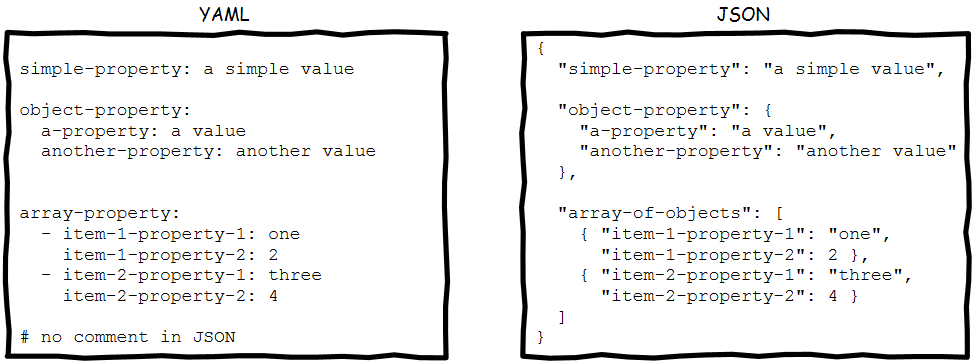
\includegraphics[width=\linewidth]{images/yaml-vs-json.png}
    \caption{Comparación de sintaxis entre YAML y JSON}
    \label{fig:yaml-vs-json}
\end{figure}

\begin{figure}[h]
    \centering
    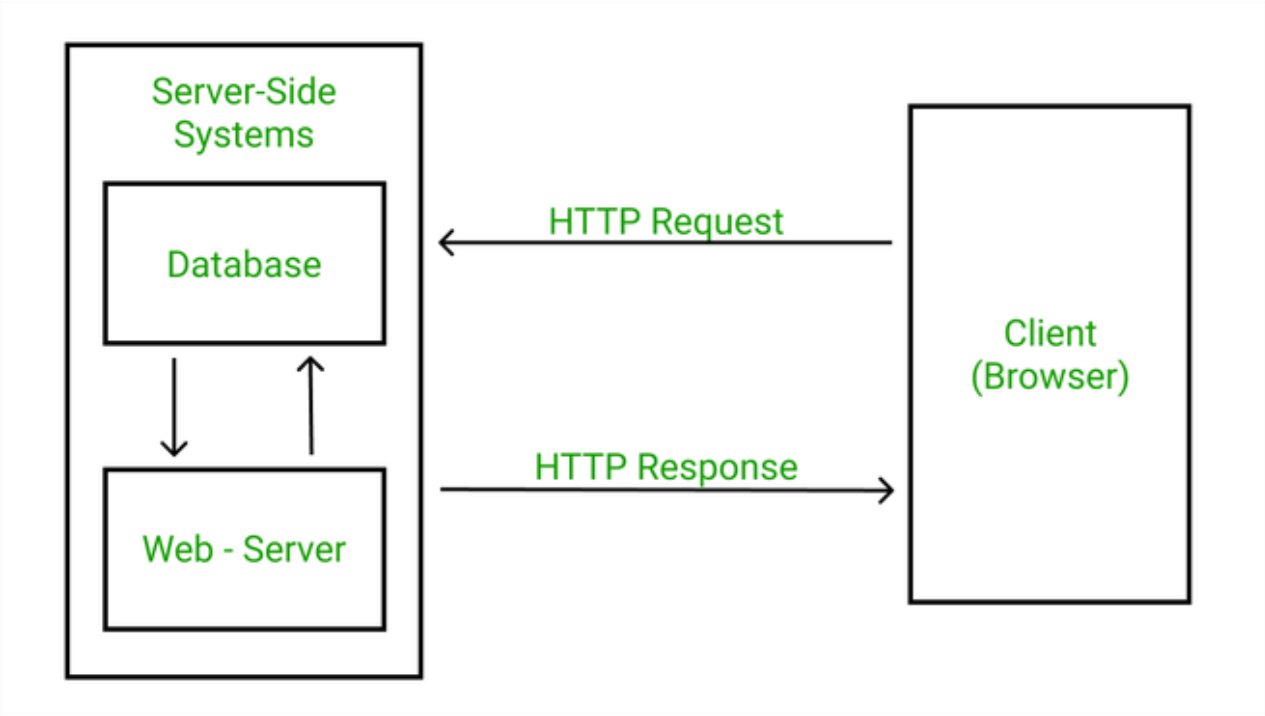
\includegraphics[width=\linewidth]{images/call-return-style.png}
    \caption{Diagrama representando el estilo arquitectónico Llamada Retorno}
    \label{fig:call-return-style}
\end{figure}

\begin{figure}[h]
    \centering
    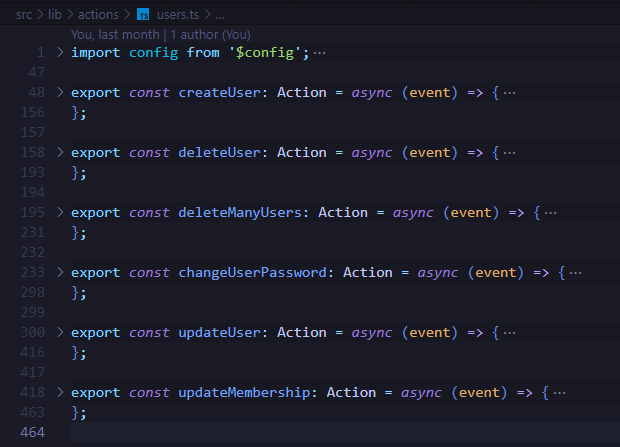
\includegraphics[scale=0.8]{images/code/collapsed-view-of-user-module.png}
    \caption{Vista colapsada del módulo de encargado de la gestión de usuarios}
    \label{fig:collapsed-view-of-user-module}
\end{figure}

\begin{figure}[h]
    \centering
    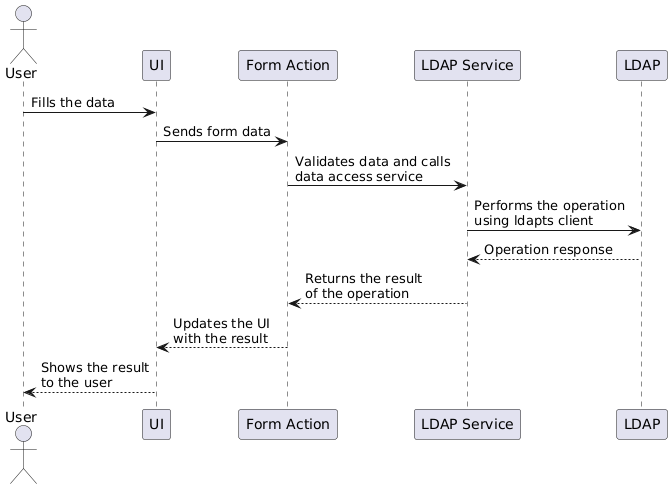
\includegraphics[width=\linewidth]{images/puml/sequence diagram form submission/sequence diagram form submission.png}
    \caption{Diagrama de sequencia mostrando un flujo de envío de formulario general}
    \label{fig:general-form-submission-diagram}
\end{figure}

\newpage
\begin{figure}[h]
    \centering
    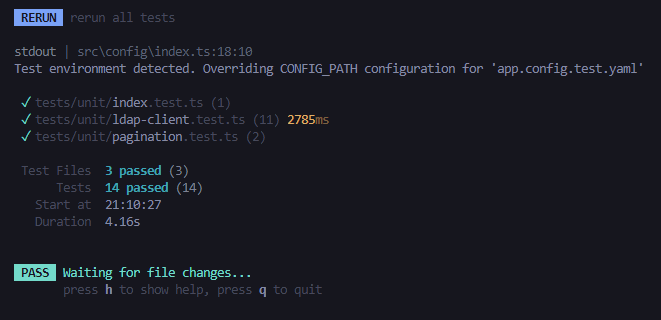
\includegraphics[width=\linewidth]{images/vitest tests run successfully.png}
    \caption{Pruebas con vitest pasaron exitosamente}
    \label{fig:integration-tests-run-ok}
\end{figure}

\begin{figure}[h]
    \centering
    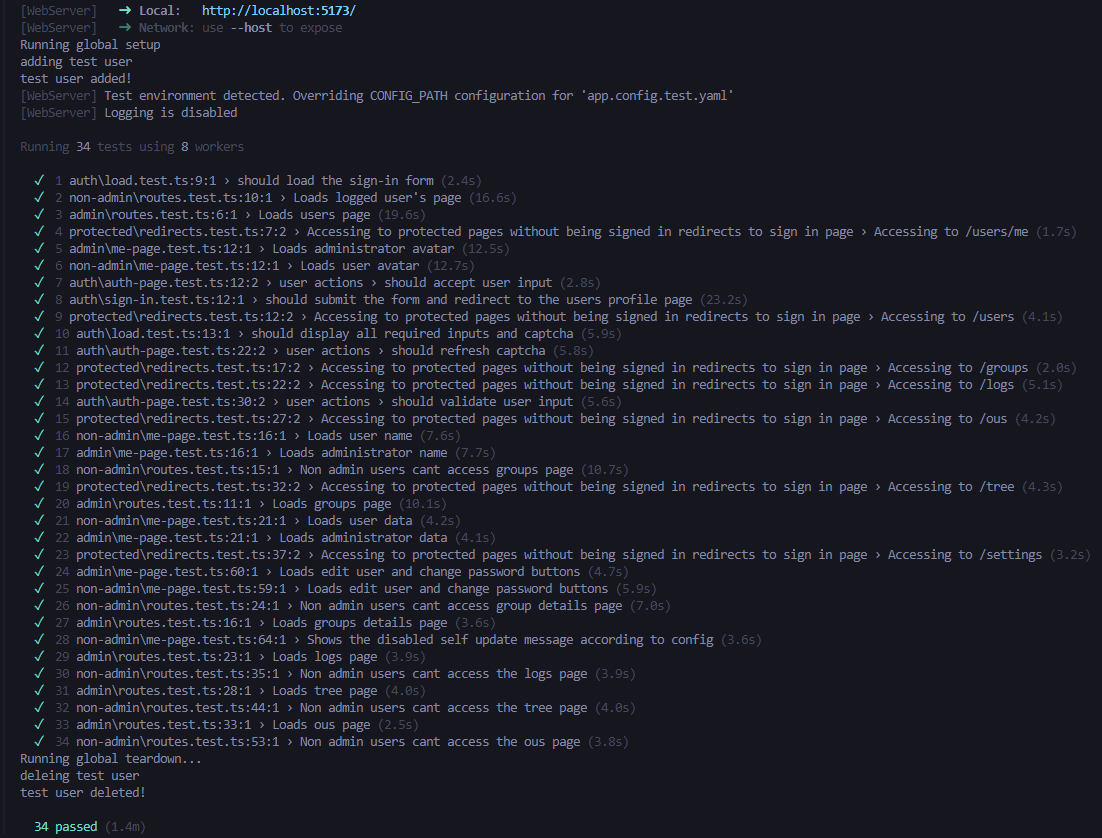
\includegraphics[width=\linewidth]{images/playwright tests run successfully.png}
    \caption{Pruebas de e2e pasaron exitosamente}
    \label{fig:e2e-test-run-ok}
\end{figure}


\begin{figure}[h]
    \centering
    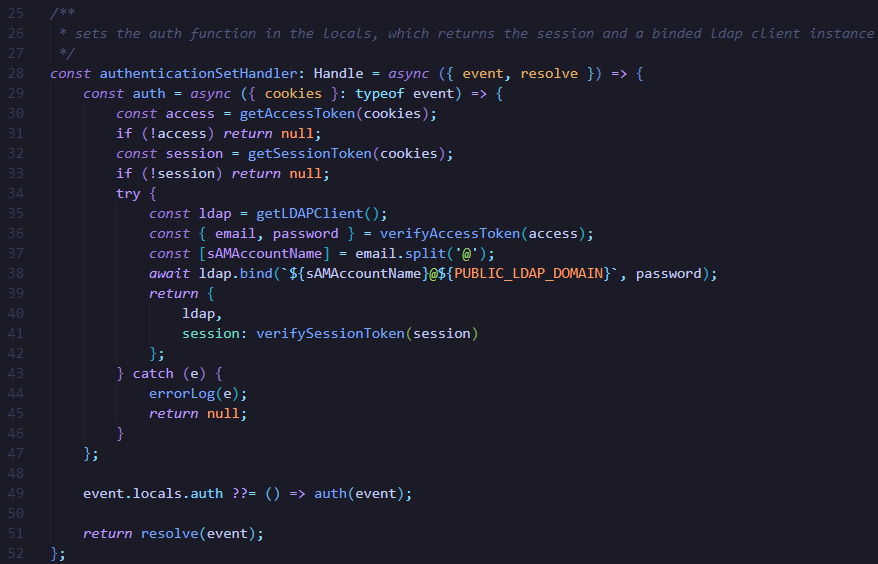
\includegraphics[width=\textwidth]{images/code/authenticationSetHandler.png}
    \caption{Manejador: autenticación y creacion del cliente LDAP}
    \label{fig:authentication-set-handler}
\end{figure}

\begin{figure}[h]
    \centering
    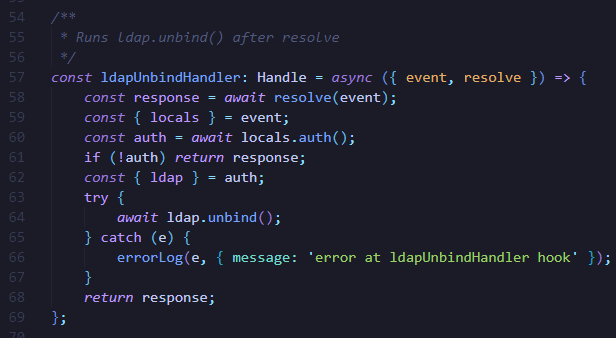
\includegraphics[width=\textwidth]{images/code/ldapUnbindHandler.png}
    \caption{Manejador: Cierre de la conexion del cliente LDAP}
    \label{fig:ldap-unbind-handler}
\end{figure}


\newgeometry{hmargin=0.5cm, vmargin=3cm}
\begin{figure}[h]
    \centering
    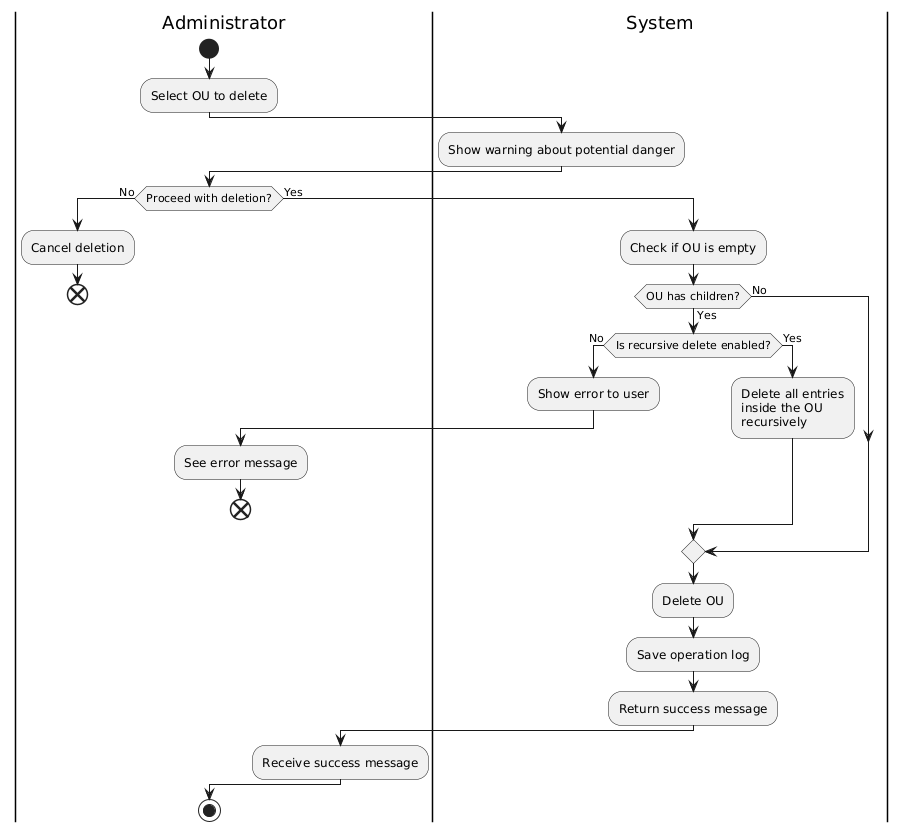
\includegraphics[width=\linewidth]{images/puml/activity-diagram delete ou/activity-diagram delete ou.png}
    \caption{Diagrama de actividades: Eliminar Unidad Organizacional}
    \label{fig:activity-diagram-delete-ou}
\end{figure}
\restoregeometry

\newpage
\newgeometry{hmargin=1cm, vmargin=3.5cm}
\begin{landscape}
    \begin{figure}
        \centering
        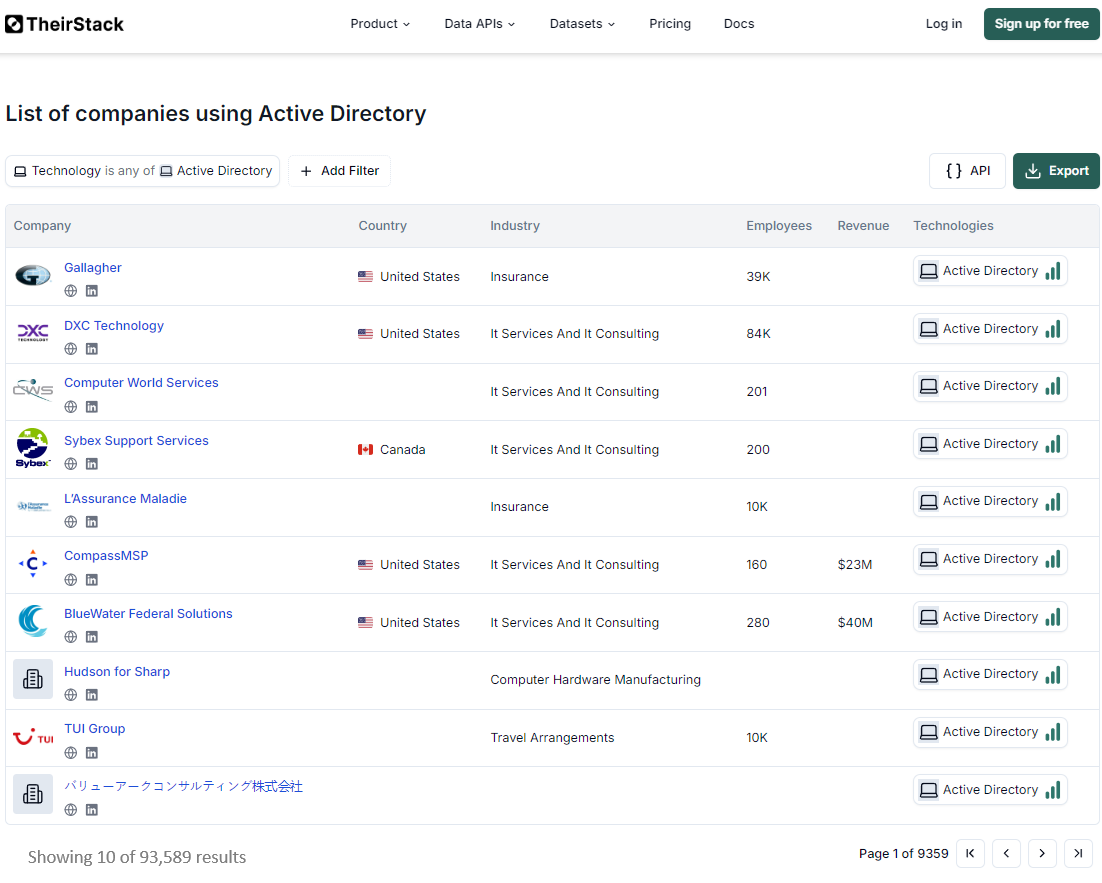
\includegraphics[width=\linewidth]{images/companies using ad - 2 .png}
        \caption{Compañías que usan Directorio Activo hoy en dia en el mundo (90 000+)}
        \label{fig:companies-using-ad}
    \end{figure}

    \begin{figure}[h]
        \centering
        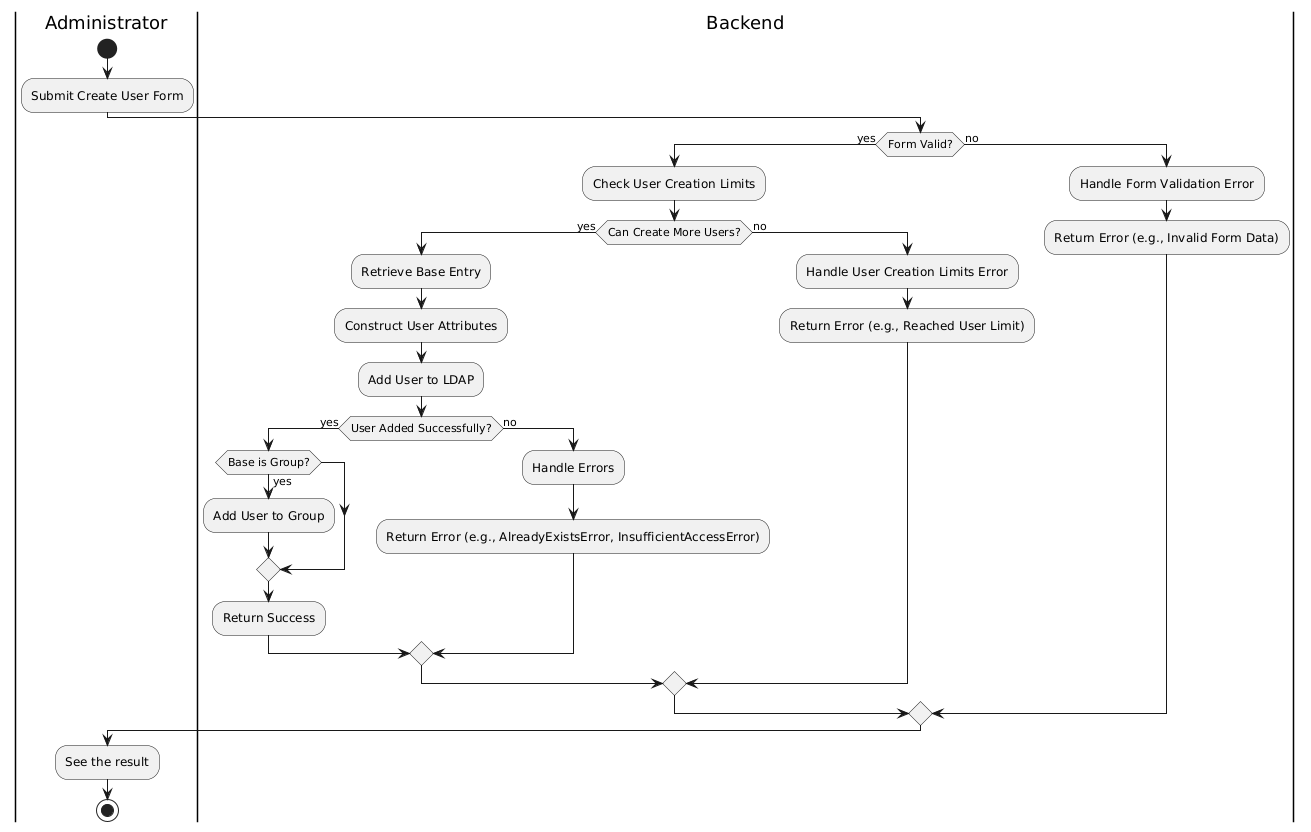
\includegraphics[scale=0.55]{images/puml/activity-diagram-create-user/activity-diagram create user.png}
        \caption{Diagrama de actividades: Crear usuario}
        \label{fig:activity-diagram-create-user}
    \end{figure}
\end{landscape}
\restoregeometry


\newgeometry{vmargin=1.5cm}
\begin{figure}[h]
    \centering
    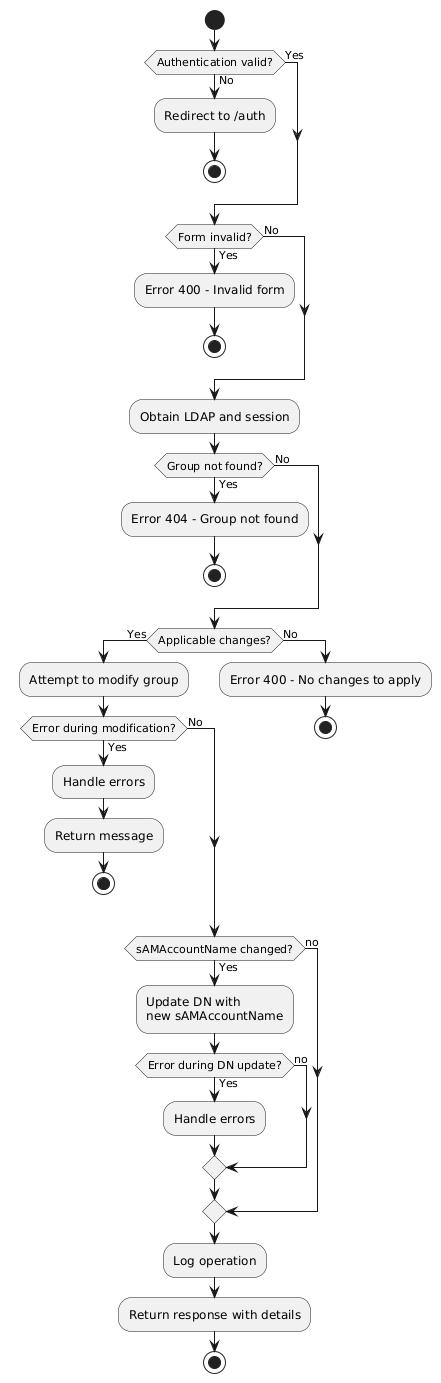
\includegraphics[height=26cm]{images/puml/flow-diagram-update group/flow-diagram update group.png}
    \caption{Diagrama de flujo: Actualizar grupo}
    \label{fig:flow-diagram-update-group}
\end{figure}
\restoregeometry

\end{document}
